\section{Introduction}\label{sec:intro}

A logistic regression that has not seen a sample, and disagrees with its label, is usually right. On digits, dropping every such sample and refitting wins back most of the mean accuracy gap that label noise opens for logistic regression (the \emph{recovered share}: filter minus noisy logistic regression, divided by clean minus noisy logistic regression, from 5-seed means). On breast cancer the same rule recovers only 22\%\src{recovery_bc_n40} of the gap at 40\%\src{noise_max_pct} noise, and its gain at 20\%\src{noise_mid_pct} noise is not significant.

Labels collected at scale are often wrong, and a linear model trained on them pays for it: at 40\%\src{noise_max_pct} symmetric noise, logistic regression loses 13.2\src{loss_digits_n40} points of test accuracy on digits. Surveys list many repairs \citep{song2023learning,frenay2014classification}. Loss correction and reweighting need an estimate of the noise rate or a clean validation set \citep{patrini2017making,ren2018learning}, and practitioners often have neither. Our two datasets are small and nearly linearly separable, and symmetric flips are the most favorable case for a linear filter, so the results below say little about harder data.

We revisit a simpler idea, out-of-fold filtering of mislabeled data \citep{brodley1999identifying}, as a baseline that needs no side information. The out-of-fold filter fits logistic regression with cross-validation, drops every training sample whose out-of-fold prediction disagrees with its label, and refits on the rest. A flipped label contradicts the structure that the other labels share. Because the prediction is out-of-fold, the model has not seen the sample it judges, which should keep it from agreeing with a flipped label. The rule is not new. What we add is a measurement: its precision and recall against known flipped labels, the recovered share, and a comparison with a multilayer perceptron (MLP).

Figure~\ref{fig:teaser} shows what this buys. The disagreement is a precise and high-recall detector: on digits at 40\%\src{noise_max_pct} noise, 76\%\src{prec_digits_n40} of dropped samples are truly flipped and 98\%\src{rec_digits_n40} of flipped labels are dropped (Fig.~\ref{fig:teaser}a). Refitting on the kept samples recovers 68\%\src{recovery_digits_n40} of the mean gap there. A sanity check with an untuned MLP trained on the same noisy labels shows that the network degrades faster (Fig.~\ref{fig:teaser}b). On clean labels the filter costs little accuracy ($-$0.2\src{gain_digits_n0_vs_logreg} points on digits, $-$0.1\src{gain_bc_n0_vs_logreg} on breast cancer, neither significant), although it drops 3.5\%\src{dropped_frac_digits_n0} and 1.9\%\src{dropped_frac_bc_n0} of the clean samples (Fig.~\ref{fig:teaser}c). It does not reach clean-label accuracy at 40\%\src{noise_max_pct} noise.

\begin{figure*}[t]
  \centering
  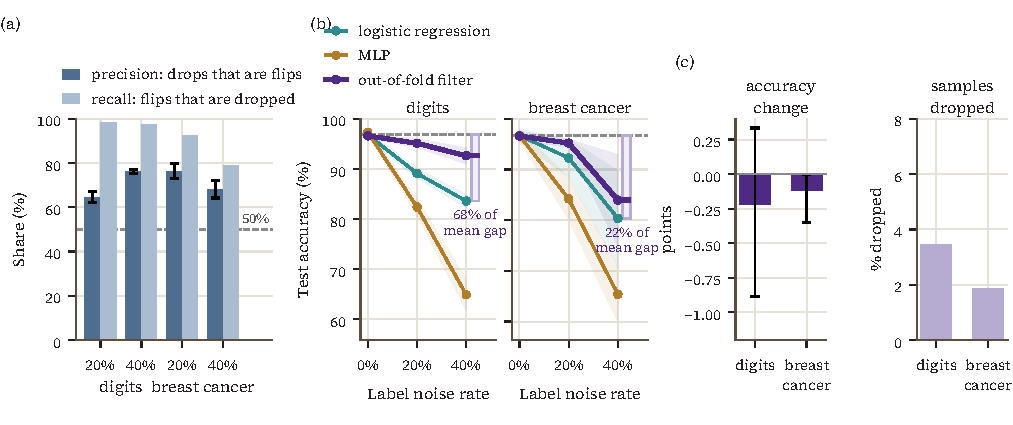
\includegraphics[width=\textwidth]{figures/teaser.pdf}
  \caption{Out-of-fold disagreement of logistic regression finds flipped labels, and dropping those samples wins back much of the mean accuracy gap that label noise opens on digits, but less on breast cancer. (a) Precision and recall of the drop set at two noise rates; the dashed line marks 50\%. (b) Test accuracy against noise for logistic regression, an untuned MLP and the out-of-fold filter; bands are sd over 5 seeds, and the box at the right edge marks the share of the mean gap won at 40\%\src{noise_max_pct} noise. (c) Cost of filtering on clean labels (no label flipped): paired accuracy change against logistic regression (95\% interval over 5 seeds) and share of clean samples dropped.}
  \label{fig:teaser}
\end{figure*}

We make three contributions.
\begin{itemize}
  \item We show that the out-of-fold disagreement of a logistic regression with a training label is a precise and high-recall detector of flipped labels on two datasets under symmetric noise.
  \item We evaluate the classical out-of-fold filter with one linear model and no side information, measuring the recovered share against noisy logistic regression.
  \item We show that it improves over logistic regression at 40\%\src{noise_max_pct} noise on both datasets and at 20\%\src{noise_mid_pct} on digits (not significant on breast cancer at 20\%\src{noise_mid_pct}), that it costs little on clean labels, and where it falls short. An untuned MLP serves as a sanity check.
\end{itemize}
